\documentclass{standalone}

\usepackage{tikz}
\usepackage{amsmath}
\usepackage{xcolor}

\definecolor{jet}{HTML}{363636}
\definecolor{outerspace}{HTML}{464646}
\definecolor{granitegray}{HTML}{616161}
\definecolor{raisinblack}{HTML}{252525}
\definecolor{tigerseye}{HTML}{EB9438}
\definecolor{denimblue}{HTML}{2B3EAB}
\definecolor{englishgreen}{HTML}{26523C}
\definecolor{upmaroon}{HTML}{780D14}
\definecolor{isabelline}{HTML}{EDEDED}
\definecolor{palmleaf}{HTML}{6DA63F}

\usetikzlibrary{shapes.arrows,chains}

\begin{document}

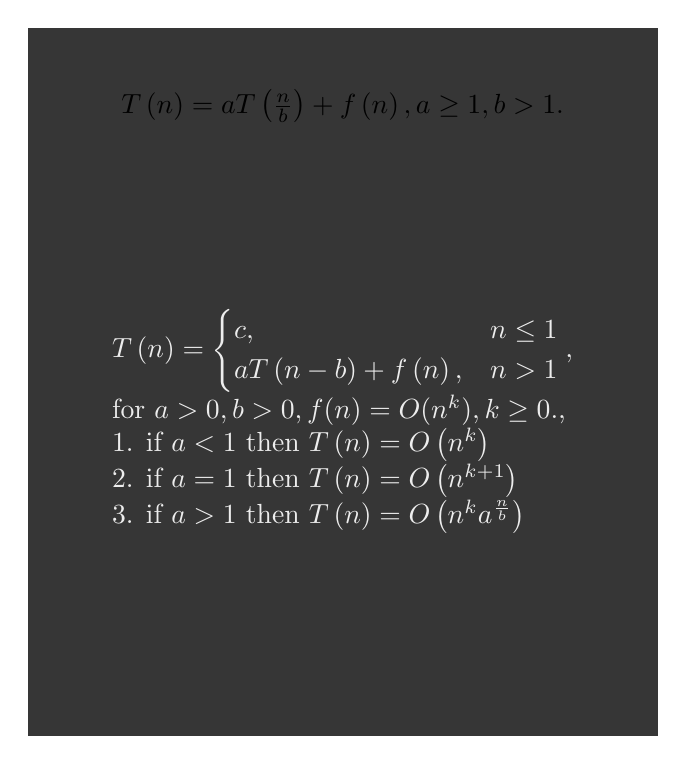
\begin{tikzpicture}
  % Background
  \fill [jet] (-4, -4) rectangle (4, 5);

  \node at(0, 4) {
    $T\left(n\right)=aT\left(\frac{n}{b}\right) + f\left(n\right), a \ge 1, b > 1.$\\
  };
  \node[align=left,text=isabelline] at(0, 0) {
    $T\left(n\right)=
        \begin{cases}
          c,& n \le 1 \\
          aT\left(n - b\right) + f\left(n\right),& n > 1
        \end{cases},$\\
     for $a > 0, b > 0, f(n) = O(n^{k}), k \ge 0.$,\\
     1. if $a<1$ then $T\left(n\right) = O\left(n^{k}\right)$\\
     2. if $a=1$ then $T\left(n\right) = O\left(n^{k + 1}\right)$\\
     3. if $a>1$ then $T\left(n\right) = O\left(n^{k}a^{\frac{n}{b}}\right)$
  };
\end{tikzpicture}

\end{document}
